\documentclass[xcolor=table]{beamer}

\usepackage{pgfpages}
\usepackage[utf8]{inputenc}
\usepackage[T1]{fontenc}
\usepackage[style=ieee]{biblatex}


\addbibresource[]{references.bib}

\usetheme[vertical,lang=en,pagenumbers]{NewPwr}

\title{Versioning filesystem with file history deduplication}
\subtitle{Wersjonowany system plików z deduplikacją historii zmian}
\author[author1]{inż. Bartłomiej Chmiel}
\institute{Faculty of Information and Communication Technology}
\date{April 14, 2023}

%footcite [1]
\makeatletter
    \def\@makefnmark{\hbox{{{\usebeamercolor[fg]{footnote mark}\usebeamerfont*{footnote mark} [\@thefnmark]}}}}

    \def\@makefntext#1{%
        \def\insertfootnotetext{ #1}%
        \def\insertfootnotemark{\@makefnmark}%
        \usebeamertemplate***{footnote}}    
\makeatother


\begin{document}

	\frame{\titlepage}

	\begin{frame}{Table of contents}
		\begin{enumerate}
			\item Introduction
			\item Literature review
			\item Areas for improvement
			\item Thesis goal
			\item Thesis scope
		\end{enumerate}
	\end{frame}

	\begin{frame}{Introduction}
		\begin{itemize}
			\item What is a filesystem?
			\item What is a versioning filesystem?
			\item What is a data deduplication?
			\item How deduplication works in a filesystem?
		\end{itemize}
	\end{frame}

	\begin{frame}{Introduction --- What is a filesystem?}
		
	\end{frame}

	\begin{frame}{Introduction --- What is a versioning filesystem?}
		
	\end{frame}

	\begin{frame}{Introduction --- What is a data deduplication}
		\begin{figure}
			\centering
			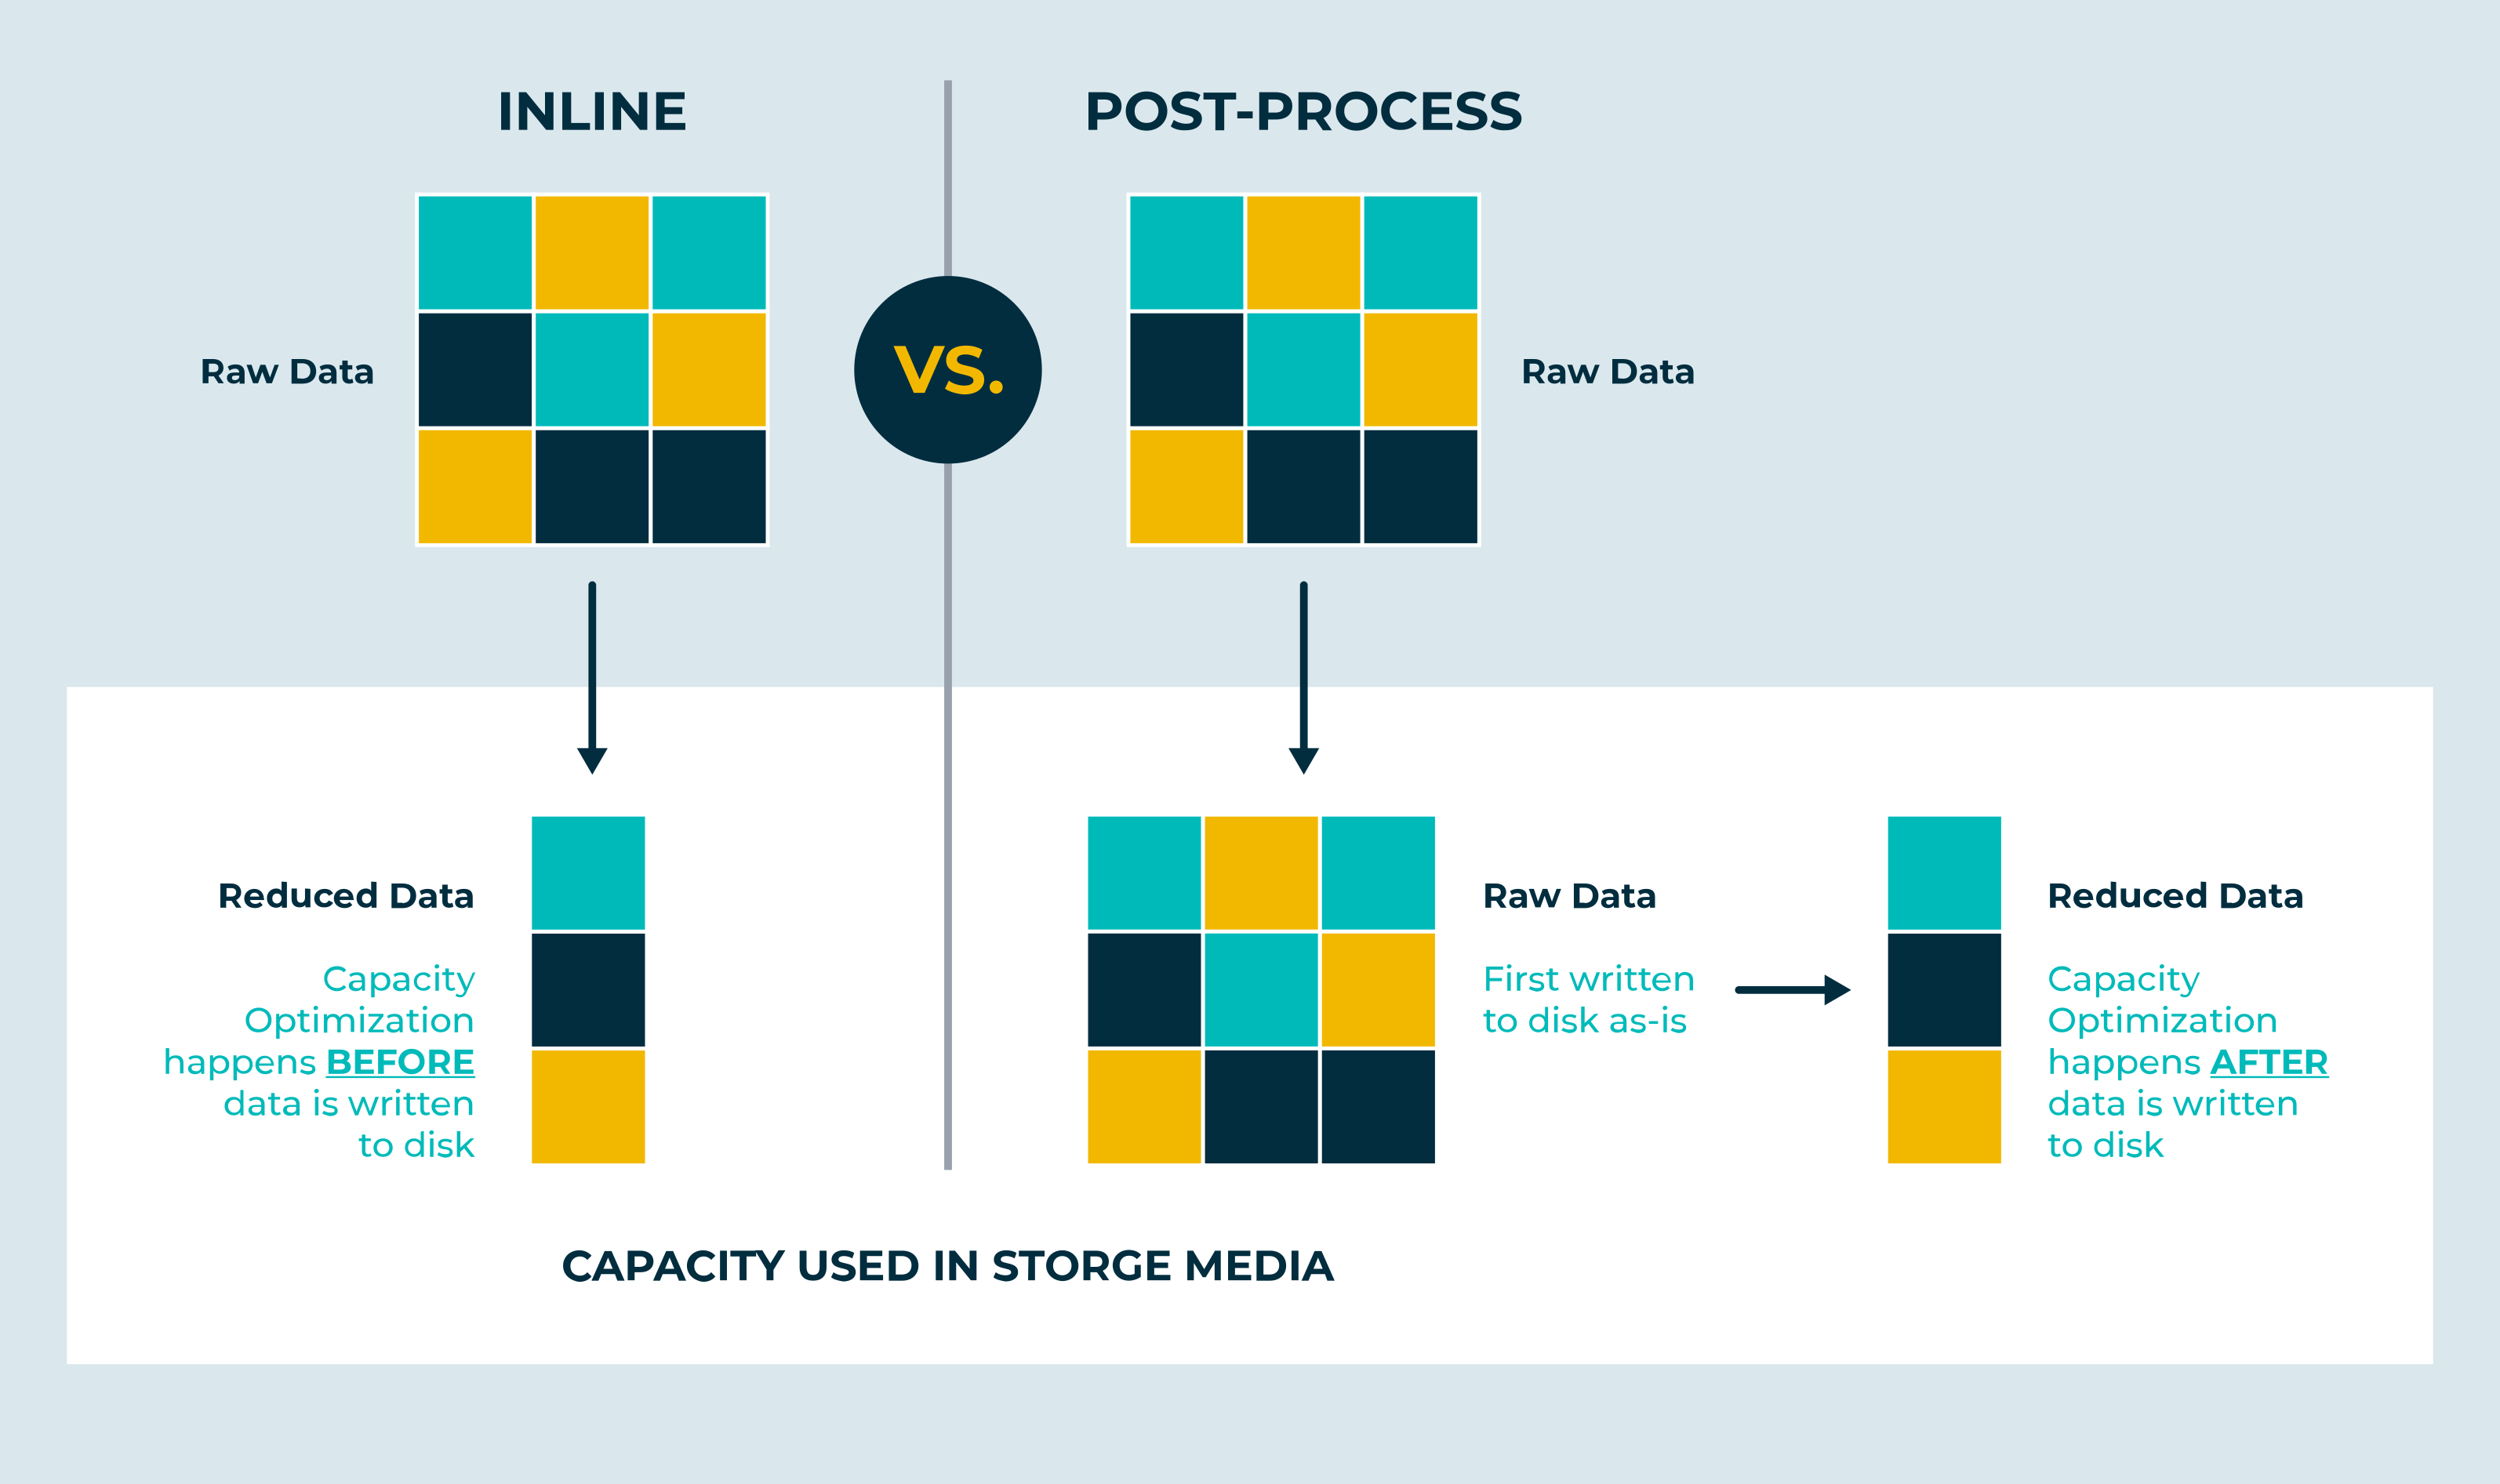
\includegraphics[width=\textwidth]{media/dedup-types.png}
			\caption{Data deduplication types\footfullcite{DedupTechTarget}}
		\end{figure}
	\end{frame}

	\begin{frame}{Introduction --- ?}
			
	\end{frame}

	\begin{frame}{Literature review}
		\begin{itemize}
			\item The NILFS filesystem
			\item The ZFS filesystem
			\item The Btrfs filesystem
			\item The CopyFS filesystem
			\item The Wayback filesystem
		\end{itemize}	
	\end{frame}

	\begin{frame}{The NILFS filesystem}
		\begin{figure}
			\centering

			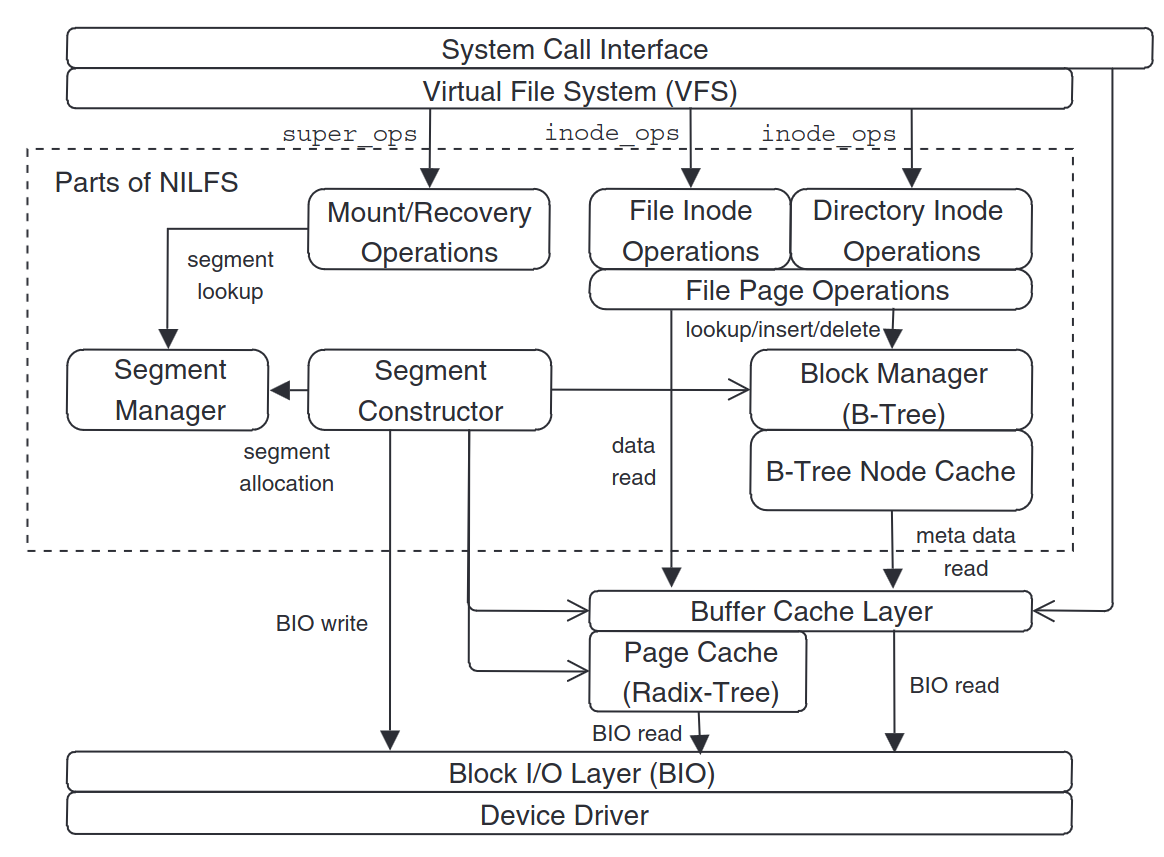
\includegraphics[width=0.9\textwidth]{media/nilfs.png}
			\caption{The block diagram of the NILFS filesystem \footfullcite{LinuxLogStructuredFileSystem}}
			\label{fig:nifls}
		\end{figure}	
	\end{frame}

	\begin{frame}{The ZFS filesystem}
		\begin{figure}
			\centering

			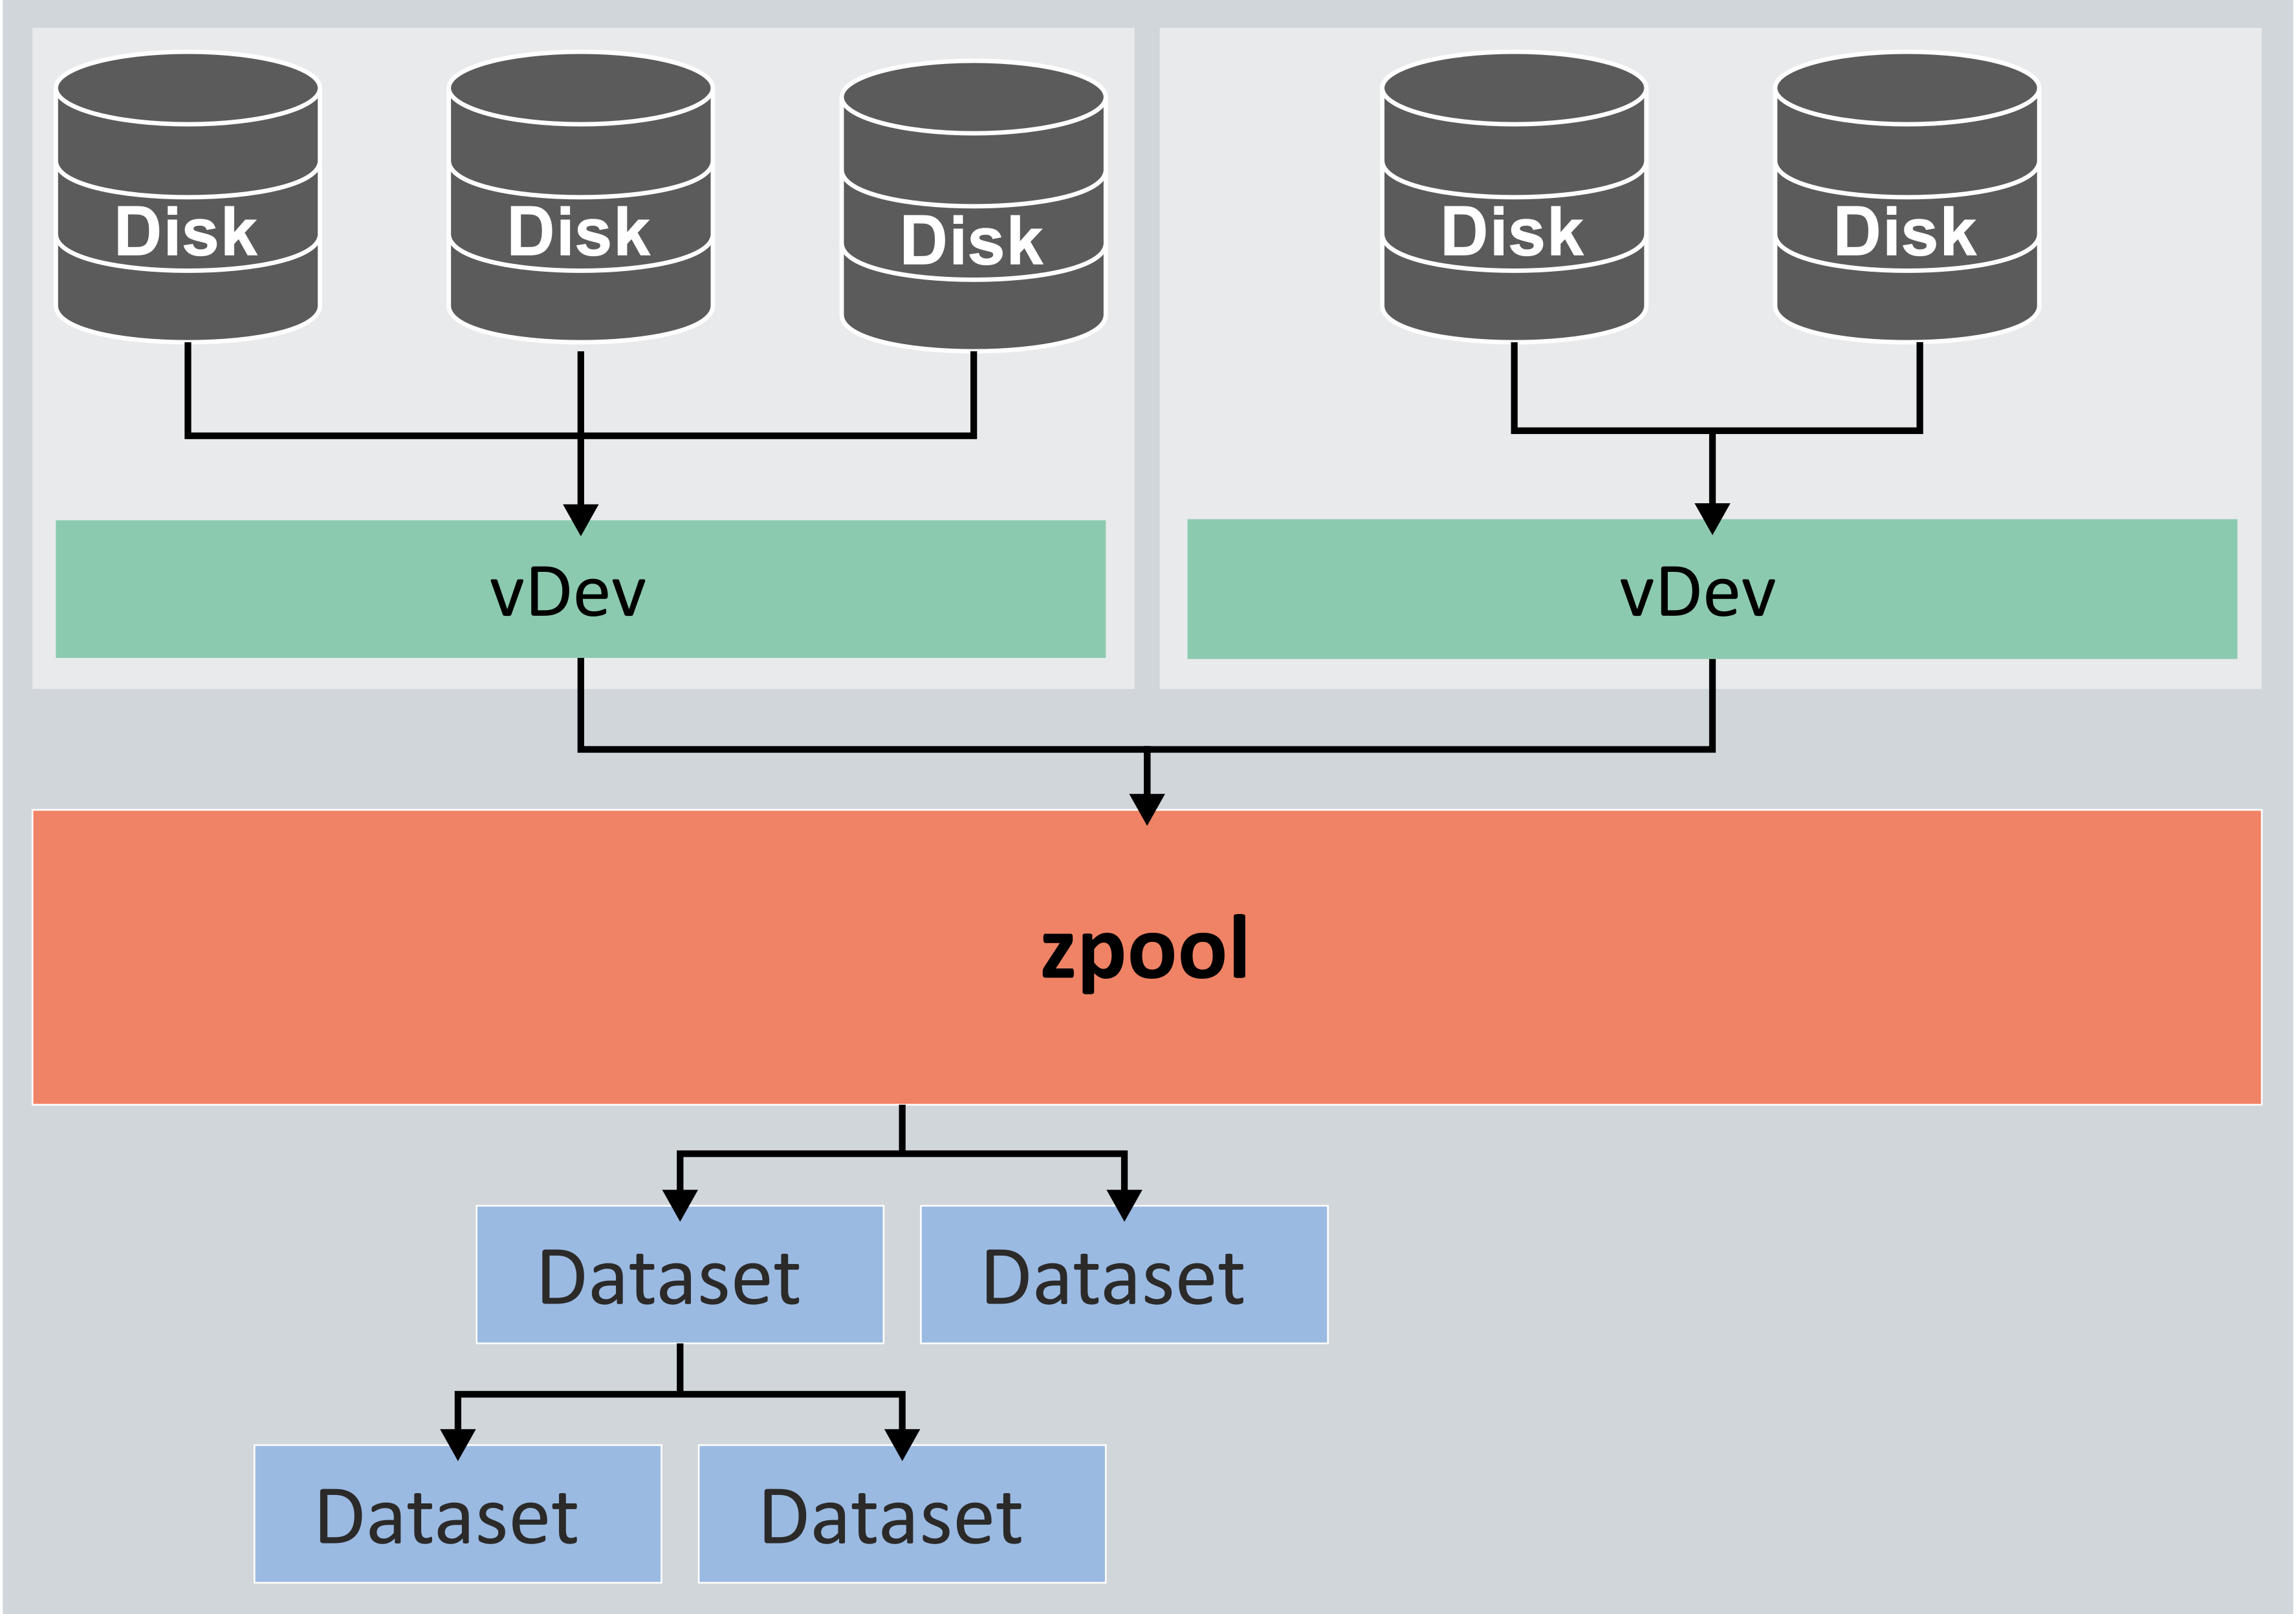
\includegraphics[width=\textwidth]{media/zfs.png}
			\caption{The structure of the ZFS filesystem \footfullcite{ZfsStructure}}
			\label{fig:zfs}
		\end{figure}
		
	\end{frame}

	\begin{frame}{The Btrfs filesystem}
		\begin{figure}
			\centering

			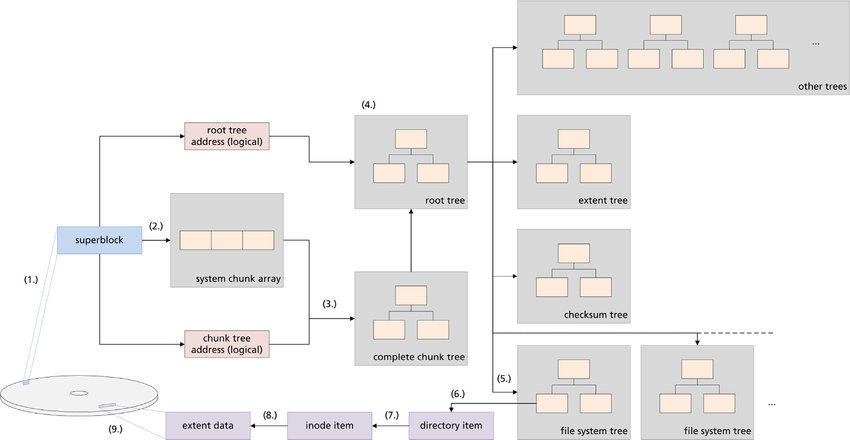
\includegraphics[width=\textwidth]{media/btrfs.png}
			\caption{The structure of the Btrfs filesystem \footfullcite{BtrfsStructure}}
			\label{fig:btrfs}
		\end{figure}
			
	\end{frame}

	\begin{frame}{The CopyFS filesystem}
		\begin{figure}
			\centering

			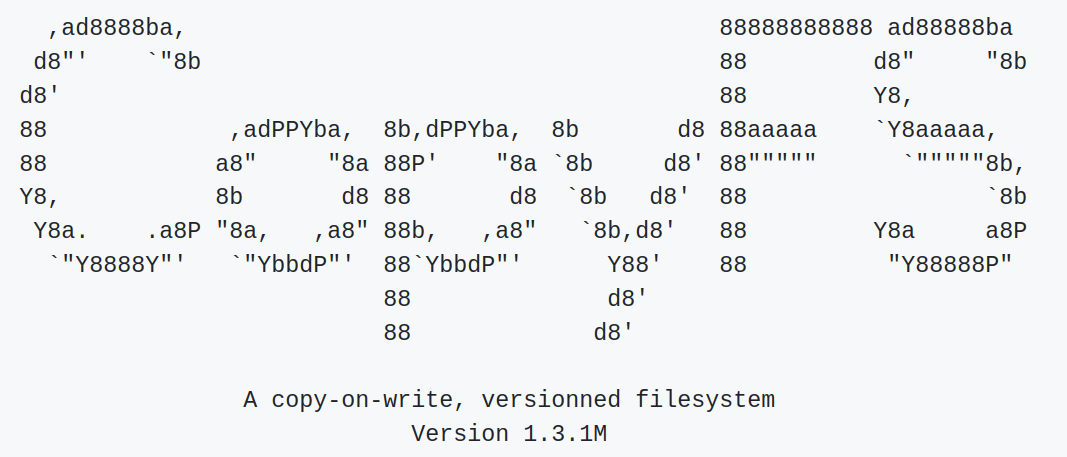
\includegraphics[width=\textwidth]{media/copyfs.png}
			\caption{Excerpt from CopyFS README \footfullcite{Copyfs}}
			\label{fig:copyfs}
		\end{figure}
		
	\end{frame}

	\begin{frame}{The Wayback filesystem}
		\begin{figure}
			\centering

			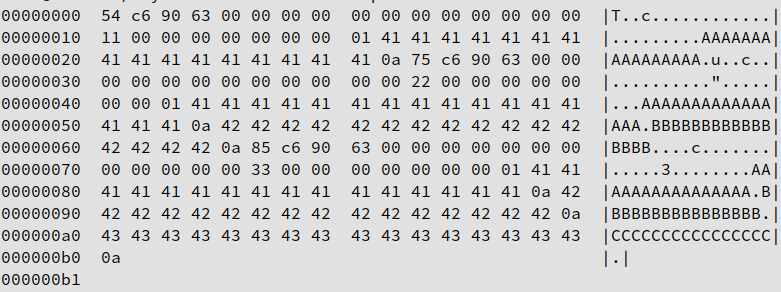
\includegraphics[width=\textwidth]{media/waybackfs-history.png}
			\caption{Wayback versioning file preview (own work)}
			\label{fig:wayback_versioning_history}
		\end{figure}
	\end{frame}

	\begin{frame}{Thesis goal}
		\begin{block}{Thesis goal}
			The goal is to analyse the methods for change history deduplication in 
			versionned filesystems in Linux environment. 

			Those methods will be analysed regarding their memory efficiency.
		\end{block}
	\end{frame}
	\note{
		Celem pracy jest analiza metod deduplikacji historii zmian w wersjonowanych 
		systemach plików w środowisku Linux. Metody deduplikacji będą analizowane 
		pod kątem wydajności pamięciowej.
	}

	\begin{frame}{Thesis scope}
		\begin{itemize}
			\item Literature review and internal structure analysis of versionned filesystems.
			\item Analysis of methods for change history deduplication in versionned filesystems.
			\item Design and implementation of a method for change history deduplication in versionned filesystem.
			\item Comparative analysis of obtained solution and methods analysed
			during literature review
		\end{itemize}
	\end{frame}
	\note{
		Zakres pracy obejmuje następujące zagadnienia:
			--- Przegląd literatury i zapoznanie się z istniejącymi technologiami budowy
			wersjonowanych systemów plików oraz publikacjami dotyczącymi
			deduplikacji historii zmian w tychże systemach.

			--- Analiza rozwiązań służących deduplikacji historii zmian w
			wersjonowanych systemach plików.

			--- Opracowanie oraz implementacja metody deduplikacji historii zmian w
			wersjonowanym systemie plików.

			--- Analiza porównawcza otrzymanego rozwiązania z metodami analizowanymi
			podczas przeglądu literaturowego
	}

	\begin{frame}{References}
		\printbibliography
	\end{frame}

\end{document}
